%%%%%%%%%%%%%%%%%%%%%%%%%%%%%%%%%%%%%%%%%
% Stylish Article
% LaTeX Template
% Version 2.1 (1/10/15)
%
% This template has been downloaded from:
% http://www.LaTeXTemplates.com
%
% Original author:
% Mathias Legrand (legrand.mathias@gmail.com) 
% With extensive modifications by:
% Vel (vel@latextemplates.com)
%
% License:
% CC BY-NC-SA 3.0 (http://creativecommons.org/licenses/by-nc-sa/3.0/)
%
%%%%%%%%%%%%%%%%%%%%%%%%%%%%%%%%%%%%%%%%%

%----------------------------------------------------------------------------------------
%	PACKAGES AND OTHER DOCUMENT CONFIGURATIONS
%----------------------------------------------------------------------------------------

\documentclass[fleqn,10pt]{SelfArx} % Document font size and equations flushed left

\usepackage[english]{babel} % Specify a different language here - english by default

\usepackage{lipsum} % Required to insert dummy text. To be removed otherwise
\usepackage{graphicx}
\graphicspath{ {./img/} }
\usepackage{float}
\usepackage{hyperref}
%----------------------------------------------------------------------------------------
%	COLUMNS
%----------------------------------------------------------------------------------------

\setlength{\columnsep}{0.55cm} % Distance between the two columns of text
\setlength{\fboxrule}{0.75pt} % Width of the border around the abstract

%----------------------------------------------------------------------------------------
%	COLORS
%----------------------------------------------------------------------------------------

\definecolor{color1}{RGB}{0,0,90} % Color of the article title and sections
\definecolor{color2}{RGB}{0,20,20} % Color of the boxes behind the abstract and headings

%----------------------------------------------------------------------------------------
%	HYPERLINKS
%----------------------------------------------------------------------------------------

\usepackage{hyperref} % Required for hyperlinks
\hypersetup{hidelinks,colorlinks,breaklinks=true,urlcolor=color2,citecolor=color1,linkcolor=color1,bookmarksopen=false,pdftitle={Title},pdfauthor={Author}}

%----------------------------------------------------------------------------------------
%	ARTICLE INFORMATION
%----------------------------------------------------------------------------------------

\JournalInfo{Introduction to Data Analysis  and Mining 2022} % Journal information
\Archive{} % Additional notes (e.g. copyright, DOI, review/research article)

\PaperTitle{House Price Regression, Regression Report} % Article title

\Authors{Ashok Kamath and Daeyeop Kim\textsuperscript{1}*} % Authors
\affiliation{\textsuperscript{1}\textit{Computer Science, School of Informatics , Computing and Engineering, Indiana University, Bloomington, IN, USA}} % Author affiliation


\Keywords{House --- Prices --- Prediction} % Keywords - if you don't want any simply remove all the text between the curly brackets
\newcommand{\keywordname}{Keywords} % Defines the keywords heading name

%----------------------------------------------------------------------------------------
%	ABSTRACT
%----------------------------------------------------------------------------------------

\Abstract{In this project, we want to predict the sale prices of housing. }

%----------------------------------------------------------------------------------------

\begin{document}

\flushbottom % Makes all text pages the same height

\maketitle % Print the title and abstract box

\tableofcontents % Print the contents section

\thispagestyle{empty} % Removes page numbering from the first page




%----------------------------------------------------------------------------------------
%Problem and Data Description
%----------------------------------------------------------------------------------------


\section{Problem and Data Description} % The \section*{} command stops section numbering

For the housing prices dataset, the problem is predicting the sale prices of the houses and the objective is to use the attributes in the dataset to predict the sale price. 

For this dataset, the training set has 1460 rows and 81 columns while the test set has 1459 rows and 80 columns. Therefore, the train-test-split ratio is about 50-50. 

The columns describe features of each house such as the Overall Quality, the neighborhood, land slope, year built, roof style, bedroom, kitchen, and gross living area. Since there are so many columns, it could be productive to find the columns that are most correlated with Sale Price and use those in regression. 

To be more specific about the meaning of some ambiguous columns, Overall Quality refers to the overall finish and material quality while Basement Exposure refers to whether the basement is walkout or garden level. 

\bigskip
\bigskip

%----------------------------------------------------------------------------------------
%	Data Preprocessing $\&$ Exploratory Data Analysis
%----------------------------------------------------------------------------------------

\section{Data Preprocessing $\&$ Exploratory Data Analysis} % The \section*{} command stops section numbering

\subsection{Handling Missing Values}
Since the number of columns was so high, we decided to first find the columns that were the most correlated with sale price and only work with those columns for prediction. For that reason, we only need to handle the missing values in that subset of columns. 

After finding the columns with the greatest correlation to Sale Price, we had only two attributes that had missing values, Garage Year Built and Masonry Veneer Area, which had 81 and 8 missing values respectively. From there, we looked at the distribution of both attributes to choose the most reasonable method of filling the missing values. For Garage Year Built, the average and the median are about the same, so either would work and we chose to use the mean. For Masonry Veneer Area, the median was 0 while the mean was 103, indicating a right skewed distribution, so it made sense to fill the missing values with the median, 0. 

\bigskip
\bigskip

\subsection{Exploratory Data Analysis}
To further analyze the relationships between Sale Price and the subset of columns that had high correlation with Sale Price, we chose to create scatter plots. 
\begin{figure}[H]
    \centering
    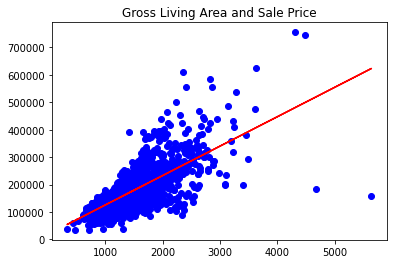
\includegraphics[width=7cm, height=6cm]{img/GrLivAreascatter.png}
    \caption{Scatter plot of Gross Living Area with Sale Price}
    \label{fig:my_label}
\end{figure}
The first scatter plot shows that Gross Living Area and Sale Price have a strong positive relationship, but there are some outliers with high gross living area yet they have a low sale price. 
\begin{figure}[H]
    \centering
    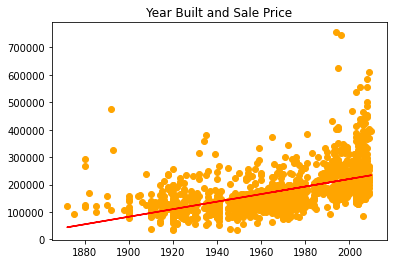
\includegraphics[width=7cm, height=6cm]{img/YearBuiltscatter.png}
    \caption{Scatter plot of Gross Living Area with Sale Price}
    \label{fig:my_label}
\end{figure}
The second scatter plot, which shows the relationship between Year Built and Sale Price, indicates a slight positive relationship between the two variables.
\begin{figure}[H]
    \centering
    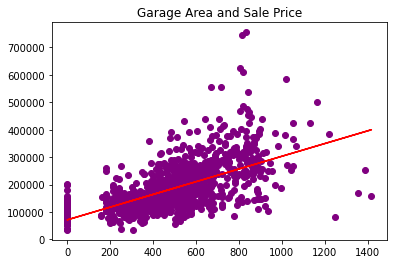
\includegraphics[width=7cm, height=6cm]{img/GrarageAreascatter.png}
    \caption{Scatter plot of Garage Area with Sale Price}
    \label{fig:my_label}
\end{figure}
The third scatter plot shows that Garage Area and Sale Price have a stronger positive relationship than Year Built but not as strong as between Gross Living Area and Sale Price.
\begin{figure}[H]
    \centering
    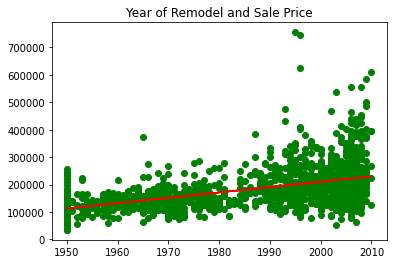
\includegraphics[width=7cm, height=6cm]{img/YearofRemodelscatter.png}
    \caption{Scatter plot of Year of Remodeling with Sale Price}
    \label{fig:my_label}
\end{figure}
The Year of Remodeling has the weakest positive relationship with Sale Price of the 4 scatter plots. 

\begin{figure}[H]
    \centering
    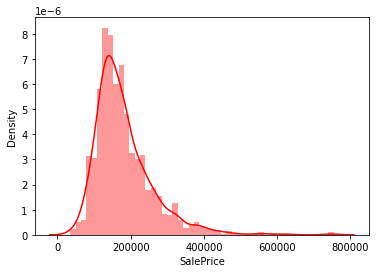
\includegraphics[width=7cm, height=6cm]{img/saleshist.png}
    \caption{Sales price distribution}
    \label{fig:my_label}
\end{figure}
We also wanted to see the distribution of some of the attributes that were included in the subset of the data we selected earlier. For Sale Price, we found the data is mostly normally distributed with a slight right skew and gross living area had a similar distribution, which would likely explain the strong correlation between the two variables. 

\begin{figure}[H]
    \centering
    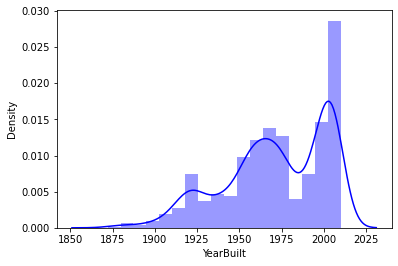
\includegraphics[width=7cm, height=6cm]{img/yrbthist.png}
    \caption{Year Built distribution}
    \label{fig:my_label}
\end{figure}
Year Built had a distribution that was left skewed. There were very few houses that were built in the 19th century and most were built after 1950. There were many houses that were built after 2000. The latest a house was built was 2010 and the earliest was 1872. 
\begin{figure}[H]
    \centering
    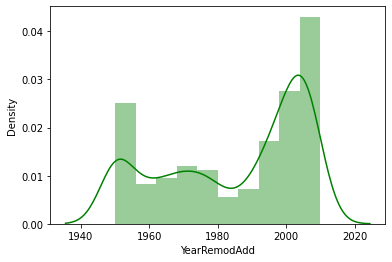
\includegraphics[width=7cm, height=6cm]{img/YearRemodhist.png}
    \caption{Year Remodeling distribution}
    \label{fig:my_label}
\end{figure}
The Year of the Remodeling tended to be either quite recent or quite old, as far back as earlier than 1960. The mean year of remodeling was 1985 while the mean was 1994. 
\begin{figure}[H]
    \centering
    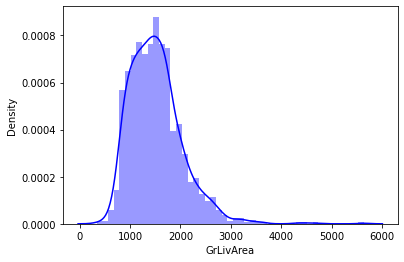
\includegraphics[width=7cm, height=6cm]{img/GriLivAreahis.png}
    \caption{Gross Living Area distribution}
    \label{fig:my_label}
\end{figure}
The Gross Living Area has a distribution that is right skewed. There were lots of data points from 500 to 3000 . 
\begin{figure}[H]
    \centering
    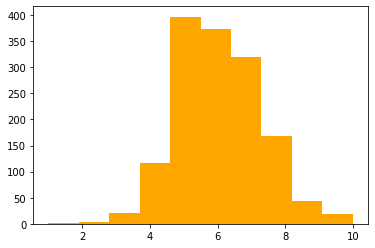
\includegraphics[width=7cm, height=6cm]{img/Overallhis.png}
    \caption{Overall Quality distribution}
    \label{fig:my_label}
\end{figure}
Overall Quality was normally distributed with the median and mean at 6. 
\begin{figure}[H]
    \centering
    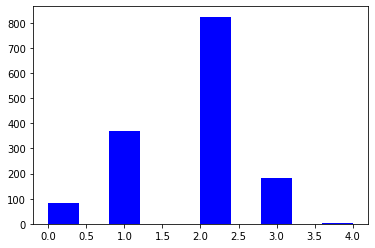
\includegraphics[width=7cm, height=6cm]{img/GraageCarshist.png}
    \caption{Garage Cars distribution}
    \label{fig:my_label}
\end{figure}
For Garage Cars, the data was normally distributed but with a slight left skew since the mean was slightly less than the mean. The maximum number of Garage Cars was 4 while some houses had no Garage Cars.
\begin{figure}[H]
    \centering
    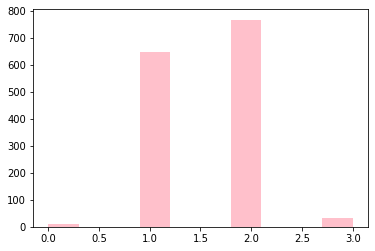
\includegraphics[width=7cm, height=6cm]{img/Fullbathhist.png}
    \caption{Full Bath distribution}
    \label{fig:my_label}
\end{figure}
For Full Bath, at least 50 percent of houses had at least 2 while some had none and the maximum number of full baths was 3. 
\begin{figure}[H]
    \centering
    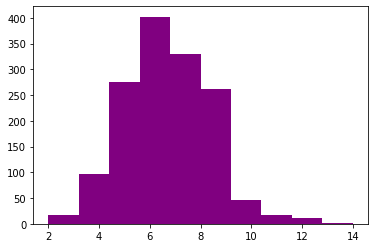
\includegraphics[width=7cm, height=6cm]{img/TotRmshist.png}
    \caption{Total Rooms Above Ground distribution}
    \label{fig:my_label}
\end{figure}
Additionally, Total Rooms Above Ground was normally distributed with the maximum being 14 and the minimum being 2. The data was slightly right skewed since the mean was 6.5 and the media was 6. 

\begin{figure}[H]
    \centering
    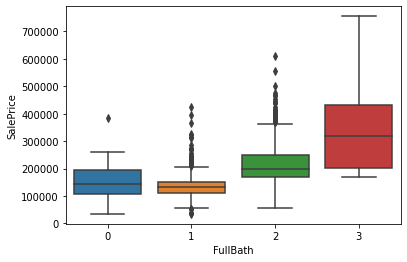
\includegraphics[width=7cm, height=6cm]{img/fullbathboxplot.png}
    \caption{Boxplots of Full Bath with Sales price}
    \label{fig:my_label}
\end{figure}
Furthermore, our boxplots indicate that with more Full Baths, the price of the house likely increases. However, there is a lot of variance when the house has 3 baths and there are outliers that could affect regression results when there are 0, 1, or 2 baths. 
\begin{figure}[H]
    \centering
    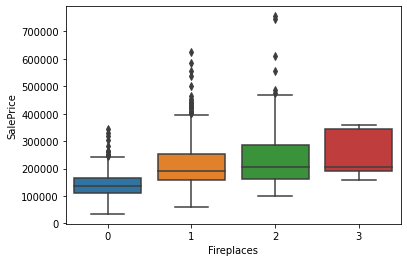
\includegraphics[width=7cm, height=6cm]{img/fireplacesboxplot.png}
    \caption{Boxplots of Fireplace with Sales price}
    \label{fig:my_label}
\end{figure}
For Fireplaces, on the other hand, when there are 3, there is not much variance in the sale price, but there is a strong right skew. For 0, 1 and 2 Fireplaces, the data is more evenly distributed, but there are more outliers. 
\begin{figure}[H]
    \centering
    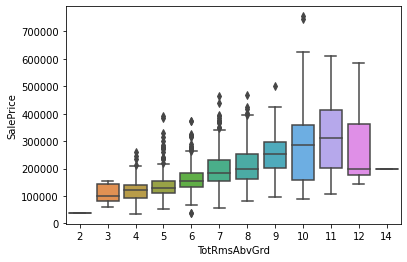
\includegraphics[width=7cm, height=6cm]{img/totrmsabvgrdboxplot.png}
    \caption{Boxplots of Total Rooms Above Ground with Sales price)}
    \label{fig:my_label}
\end{figure}
For the Total Rooms Above Ground attribute, there is hardly any variance in Sale Price when there are only 2 or 14 rooms above ground, which is probably due to a lack of entries with this number of rooms above ground. The boxplots indicate that as the total rooms above ground increases, the Sale Price typically will increase. For rooms above ground ranging from 4-10, there are outliers on the positive side. 
\begin{figure}[H]
    \centering
    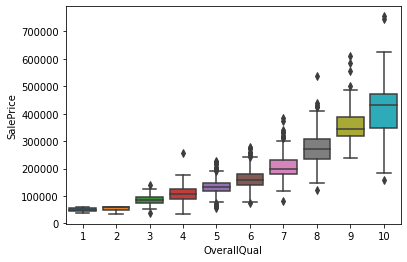
\includegraphics[width=7cm, height=6cm]{img/overallqualboxplot.png}
    \caption{Boxplots of Overall Quality with Sales price)}
    \label{fig:my_label}
\end{figure}
Finally, Overall Quality has a strong positive relationship with Sale Price. There is little variance in price when the Overall Quality is 1,2, or 3, but the variance in price increases as the Overall Quality increases. 

\bigskip
\bigskip

%----------------------------------------------------------------------------------------
 % Algorithm and Methodology
%----------------------------------------------------------------------------------------


\section{Algorithm and Methodology}

For predicting the sale prices of housing, we used linear regression to start. This algorithm works by minimizing the sum of squared errors when creating a line of best fit through the training data. The line of best fit for the training data is then used to predict the appropriate values for the entries in the testing data. 

In addition to linear regression, we used a random forest regressor, which is similar to the random forest classifier that we used on the spaceship titanic dataset. The random forest regressor, however, averages the results of the decision trees in the forest rather than take the majority vote. We also used a support vector regressor which attempts to predict new entries by first projecting the data into a higher dimension. 

Besides linear regression, random forest and support vectors, we also used the gradient boosting regressor and a simple decision tree regressor. The gradient boosting regressor continually improves a decision tree model by calculating the gradient on the errors of the previous decision tree model. The decision tree regressor, as opposed to classifier, outputs a prediction by using the average of the training data in the leaf node that the decision nodes lead to based on the test entry. 

Furthermore, we used Bayesian Ridge Regression, which employs Bayesian methods to make up for insufficient or weakly distributed data. In tandem, we used Lasso Regression, which performs a shrinkage technique that makes the data values shrink towards a central point. Lastly, similar to the classifier models for spaceship titanic, we created an MLP and KNN regressor. 

\bigskip
\bigskip
%----------------------------------------------------------------------------------------
 % Experiments and Results
%----------------------------------------------------------------------------------------
\section{Experiments and Results}

Accuracy percentage with different model 
\bigskip

\begin{tabular}{ |p{4.5cm}|p{3cm}|}
\hline
\multicolumn{2}{|c|}{Threshold percentage with 9 Models} \\
\hline
Model Name& Percentage threshold \\
\hline
Linear Regression & 71.8187\% \\
Random Forest Regression	 & 81.9776\%\\
Support Vector Regressor & -5.0832\% \\
Gradient Boosting Regressor    & 84.2915\% \\
Decision Tree Regressor	 & 67.4467\%\\
Bayesian Ridge Regression & 72.1804\% \\
Lasso Regression& 71.8188\%  \\
MLP Regressor & 68.2111\% \\
KNN Regressor	 & 72.1854\%  \\
\hline
\end{tabular}
\bigskip

Out of all the models, the Gradient Boosting Regressor model performed the best with a cross validation accuracy rate of about 84.29\%. We were impressed with this rate of accuracy since most of the other models were not able to pass the 80\% threshold. This demonstrates why the Gradient Boosting algorithm has been so popular within the data science community lately. 

The only other model that was able to pass the 80\% threshold was the random forest regressor model, which for cross validation on the training data had an accuracy rate of about 82\%. This was another model that has its foundations in decision trees, except random forest is not as strategic in improving performance with the creation of each new decision tree, which could explain why it was not as accurate as the Gradient Boosting Regressor. 

The KNN Regressor and the Bayesian Ridge Regressor had accuracies slightly above 72\% while Lasso and Linear Regression models had accuracies that were slightly below 72\%. The MLP Regressor had an accuracy of about 69\% for the training data in cross validation while the decision tree model had an accuracy of about 64\%. Lastly, the support vector regressor in cross validation failed to report a reasonable accuracy rate. 

Since the Gradient Boosting Regressor performed the best in cross validation, we used that model on the testing set and submitted our results to Kaggle, which reported we had an error of .15 while the best of all time submission had an error of .00. We placed on the leaderboard at 2474 out of 4130 spots on the leaderboard. 


%----------------------------------------------------------------------------------------
 % Summary and Conclusions
%----------------------------------------------------------------------------------------
\section{Summary and Conclusions}

For this section, the goal was to predict the sale prices of housing. The dataset had 80 attributes, excluding the target variable of sale price. All of the features described the house that was sold and some examples include Overall Quality, year built, roof style, number of bedrooms and gross living area. For handling the missing values in this dataset, we employed the same reasoning as we did for the Spaceship Titanic dataset. 

In our exploratory data analysis, we only worked with columns that had the greatest correlation with sale price since the number of attributes was high, so we wanted to narrow it down. We noticed a strong positive relationship between Gross Living Area and Sale Price via a scatter plot. Additionally, we found Sale Price was normally distributed but with a slight right skew, similar to the distribution for Gross Living Area. Our boxplots showed that a house with more Full Baths will likely have a higher price, but there is more variance as the number of full baths increase. There was a similar relationship between Overall Quality and Sale Price since the variance increased as the Overall Quality increased. 

To predict the sale prices of housing, we used various models ranging from Bayesian Ridge and Lasso Regression to KNN Regression. Through cross validation on the training data, we found that the Gradient Boosting Regressor performed best so we used that on the test data, giving us an error rate of .15, which had us place at 2474 out of 4130 spots on the leaderboard while the leading submission, in rank 1, had an error rate of .00. Our model could be improved not only by performing a grid search for each model, but also removing outliers, using columns besides those that are highly correlated with sale price, and other techniques. 

\bigskip
\bigskip
\bigskip    



%----------------------------------------------------------------------------------------
%	REFERENCE LIST
%----------------------------------------------------------------------------------------

\bibliographystyle{unsrt}

\bibliography{sample}

%----------------------------------------------------------------------------------------

\end{document}